\section{ISTA-rammeverket}
\label{sec:ista-rammeverket}

\citet{Harrison} påpeker at implementering av ny informasjonsteknologi (IT) i helsesektoren ofte medfører uforutsette og uønskede konsekvenser, noe som kan undergrave gitte praksiser og i verste fall være en risiko for pasientsikkerheten. Ofte vil helsepersonell skylde på teknologien for at slike konsekvenser og implementeringsfeil oppstår, til tross for at det i flere tilfeller er det sosiotekniske samspillet som har feilet. Rammeverket ISTA\footnote{Interactive SosioTechnical Analysis} er designet for å illustrere samspillet mellom ny IT, arbeidsmønstre, helsepersonell og organisasjoner. Dette samspillet innebærer komplekse interaksjoner, og kan føre til at svært ulik bruk selv av identiske systemer. Rammeverket er ment som en oppfordring til å se disse interaksjonene som muligheter for læring og forbedring, og ikke som irriterende barrierer eller tegn på motstand. Heltrukkede piler viser hvordan komponentene påvirker hverandre, mens stiplede piler illustrerer de sosiotekniske interaksjonene. Pil 2 viser interaksjonen mellom ny IT og den tekniske og fysiske infrastrukturen, og hvordan denne videre former hvordan teknologien anvendes \citep{Harrison}.

\begin{figure}[H]
\centering
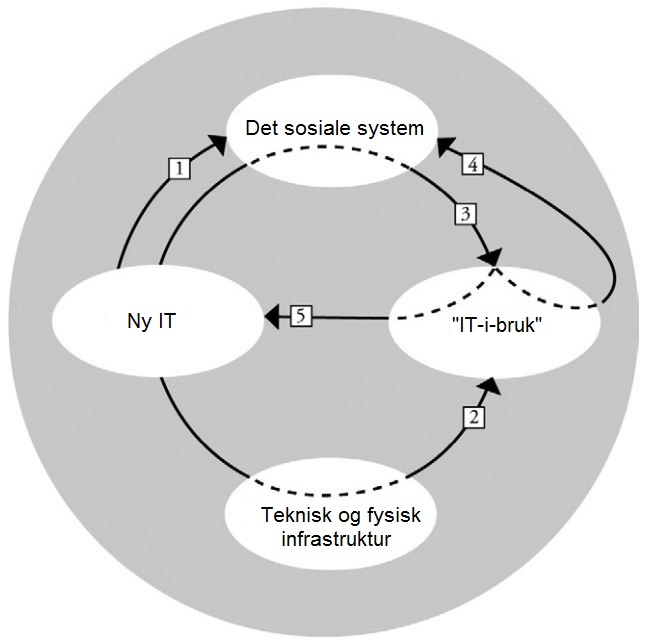
\includegraphics[scale=0.4]{ISTA.jpg}
\caption{ISTA \citep{Harrison} (oversatt av forfatterne)}
\label{fig:ISTA}
\end{figure}

\noindent
ISTA er basert på fem ulike interaksjoner mellom komponentene i et sosioteknisk system:  

\begin{enumerate}
\item Den første typen interaksjon viser hvordan ny IT endrer det eksisterende sosiale systemet, deriblant arbeidsmønstre, kommunikasjon og relasjon mellom helsepersonell. Teknologien kan eksempelvis føre til at helsepersonell må bruke mer tid på dokumentasjon enn tidligere, eller redusere den direkte kommunikasjonen ansikt-til-ansikt.
\item Dersom ny IT ikke er tilpasset eksisterende teknisk og fysisk infrastruktur, kan det oppstå utilsiktede konsekvenser, eksempelvis forsinkelse, tap av data og feil. Manglende tilpasning av IT til den fysiske settingen hvor den skal tas i bruk kan medføre bruk og workarounds som har negative effekter på sikkerhet, kvalitet og effektivitet. Teknologien kan eksempelvis være plassert slik at den er problematisk å aksessere eller flytte, eller befinne seg i omgivelser preget av støy og med mange mennesker tilstede. Plassering av arbeidsstasjoner trekkes frem som et poeng, da upassende plassering av denne kan redusere den direkte kommunikasjonen, og øke antall distraksjoner. 
\item Fortolkninger og tilpasninger av ny IT vil ofte føre til praksiser som skiller seg fra tenkt bruk. Denne bruken oppstår fordi det opprinnelige designet ikke reflekterer de eksisterende arbeidsmønstre og sosiale relasjoner, og workarounds oppstår som resultat av dette.
\item Den fjerde interaksjonen illustrerer at implementering av ny IT er en rekursiv prosess. Det sosiale systemet påvirker hvordan teknologien brukes, samtidig som denne bruken påvirker det sosiale systemet. Et eksempel på dette kan være at ansatte ikke bruker teknologien slik deres ledere ønsker. Hvis slik bruk vedvarer og tillates, kan det dermed oppstå en endring i maktforholdet mellom ledere og ansatte.  
\item Som et resultat av at brukere gjør lokale tilpasninger som skiller seg fra tenkt bruk, kan utviklere og ledere være tvunget til å gjøre endringer i teknologien.
\end{enumerate}


